\chapter{Példák}

\section{Sok körzőzés}
\begin{tikzExample}
    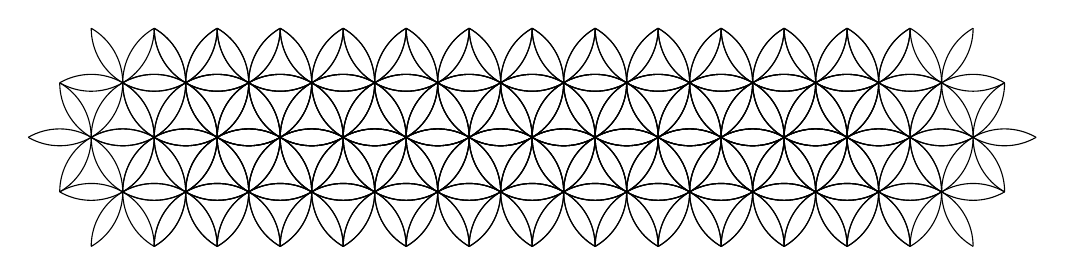
\begin{tikzpicture}[scale=0.8]
        \foreach \i in {0,...,12}
        {
            \draw (\i+0,0) circle (1);
            \draw (\i+0.5,-0.866) arc (0:120:1);
            \draw (\i+1.5,-0.866) arc (0:240:1);
            \draw (\i+-1,-0) arc (60:-60:1);
            \draw (\i+0,-1.732) arc (0:120:1);
            \draw (\i+-1.5,-0.866) arc (-120:120:1);
            \draw (\i+-1,-0) arc (-60:60:1);
            \draw (\i+-1.5,0.866) arc (-120:0:1);
            \draw (\i+0,1.732) arc (120:360:1);
            \draw (\i+0.5,0.866) arc (0:-120:1);
            \draw (\i+0.5,0.866) arc (-60:-180:1);
            \draw (\i+0.5,0.866) arc (120:240:1);
            \draw (\i+0.5,0.866) arc (180:300:1);
            \draw (\i+0.5,-0.866) arc (180:60:1);
            \draw (\i+-1,-1.732) arc (180:60:1);
            \draw (\i+1.5,0.866) arc (120:240:1);
            \draw (\i+0.5, 0.866) arc (0:60:1);
            \draw (\i+0.5, 0.866) arc (240:180:1);
            \draw (\i+0.5, 0.866) arc (240:300:1);
            \draw (\i+0.5, 0.866) arc (120:60:1);
            \draw (\i+0.5, 0.866) arc (180:120:1);
            \draw (\i+0.5, 0.866) arc (300:360:1);
            \draw (\i+-1,-0) arc (0:60:1);
            \draw (\i+-1,-0) arc (240:180:1);
            \draw (\i+-1,-0) arc (60:120:1);
            \draw (\i+-1,-0) arc (300:240:1);
            \draw (\i+-1,-0) arc (120:180:1);
            \draw (\i+-1,-0) arc (360:300:1);
            \draw (\i+0.5, -0.866) arc (180:240:1);
            \draw (\i+0.5, -0.866) arc (60:0:1);
            \draw (\i+0.5, -0.866) arc (120:60:1);
            \draw (\i+0.5, -0.866) arc (240:300:1);
            \draw (\i+0.5, -0.866) arc (120:180:1);
            \draw (\i+0.5, -0.866) arc (360:300:1);
        }    
    \end{tikzpicture}
\end{tikzExample}
    


\section{Sakktábla}
\begin{tikzExample}
    \begin{center}
        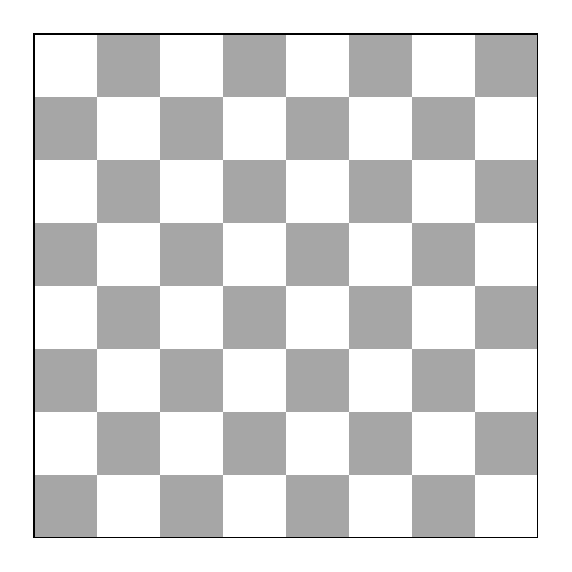
\begin{tikzpicture}[scale=0.8]
            \clip(-0.1,-0.1) rectangle (8.1,8.1);
            \foreach \i in {1,3,5,7}
                \foreach \j in {1,3,5,7}
                {
                    \fill[line width=0.pt, 		fill=gray,opacity=0.7] (\i,\j) -- (\i+1,\j) -- 	(\i+1,\j+1) -- (\i,\j+1) -- cycle;
                \fill[line width=0.pt, fill=gray,opacity=0.7] (\j,\i) -- (\j-1,\i) -- (\j-1,\i-1) -- (\j,\i-1) -- cycle;
                }
        \draw (0,0)--(0,8)--(8,8)--(8,0)--cycle;	
            \begin{Large}
                \draw (0.5,0.5) node {\bf{\symrook}};
                \draw (1.5,1.5) node {\bf{\symrook}};
                \draw (2.5,2.5) node {\bf{\symrook}};
                \draw (3.5,3.5) node {\bf{\symrook}};
                \draw (4.5,7.5) node {\bf{\symbishop}};
                \draw (5.5,7.5) node {\bf{\symbishop}};
                \draw (6.5,4.5) node {\bf{\symbishop}};
                \draw (7.5,6.5) node {\bf{\symbishop}};
            \end{Large}
        \end{tikzpicture}
        \end{center}
\end{tikzExample}

\section{}
\begin{tikzExample}

\end{tikzExample}
